\documentclass[runningheads]{llncs}
\usepackage{times}
\usepackage{amsmath}
\usepackage{amssymb}
\usepackage{algorithm}
\usepackage[noend]{algpseudocode}
%\usepackage[ruled,linesnumbered,noend,oldcommands]{algorithm2e}
\usepackage{xspace}
\usepackage{mathtools}
\usepackage{graphicx}
\usepackage{array}
\usepackage{xcolor}
\usepackage{theorem}
\usepackage[T1]{fontenc}
% \usepackage[T1,hyphens]{url}
\usepackage{hyperref}
%\PassOptionsToPackage{hypnens}{url}
\title{Clause size reduction with $i$-UIP Learning}
\author{Nick Feng \and Fahiem Bacchus}
\authorrunning{N. Feng and F. Bacchus}
\institute{Department of Computer Science, University of Toronto, Canada, 
  \email{\{nfeng,fbacchus\}@cs.toronto.edu}}

\algrenewcommand\algorithmicprocedure{}
\algrenewcommand\algorithmicthen{}
\algrenewcommand\algorithmicdo{}

\newcommand{\fs}[1]{\fontsize{#1}{#1}\selectfont}
\newcommand{\fss}[2]{\fontsize{#1}{#2}\selectfont}
\newcommand{\sat}{SAT\xspace}
\newcommand{\code}[1]{\text{#1}}
\newcommand{\inputF}{\ensuremath{F}}
\newcommand{\oneUIPClause}{\ensuremath{C_{1}}}
\newcommand{\iUIPClause}{\ensuremath{C_{i}}}
\newcommand{\assertionTrail}{\trail}
\newcommand{\LBD}{\text{LBD}}
\newcommand{\GAP}{\text{Gap}}
\newcommand{\IUIP}{\textbf{LBDstable-$i$UIP}}
\newcommand{\tryuiplevel}{\textbf{try-uip-level}\xspace}
\newcommand{\IUIPPURE}{\textbf{Pure-$i$UIP}}
\newcommand{\IUIPMIN}{\textbf{Min-$i$UIP}}
\newcommand{\IUIPGreedy}{\textbf{i-UIP-Greedy}}
\newcommand{\IUIPActive}{\textbf{i-UIP-Inclusive}}
\newcommand{\IUIPDist}{\textbf{i-UIP-Exclusive}}
\newcommand{\MapleBase}{\textit{MapleCOMSPS\_LRB}}
\newcommand{\MapleSeven}{\textit{MapleLCMDist}}
\newcommand{\MapleNine}{\textit{MapleLCMDiscChronoBT-DL-v3} }
\newcommand{\MapleEight}{\textit{MapleLCMDiscChronoBT}}
\newcommand{\MapleNineShort}{\textit{MapleCB-DL} }
\newcommand{\expSAT}{\textit{expMaple\_CM\_GCBumpOnlyLRB} }
\newcommand{\expSATShort}{\textit{expMaple} }
\newcommand{\MapleIUIPPURE}{\text{Maple-\IUIPPURE}}
\newcommand{\MapleIUIMIN}{\text{Maple-\IUIPMIN}}
\newcommand{\MapleEightShort}{\textit{MapleCB}}
\newcommand{\Set}[2]{\{\,#1\mid#2\,\}}
\newcommand{\Array}[2]{[\,#1\mid#2\,]}
\newcommand{\target}{\textbf{Succ_t}}
\newcommand{\trail}{\ensuremath{\mathcal{T}}}
\newcommand{\trailIdx}[1]{\ensuremath{\iota(#1)}}
\newcommand{\dlevel}[1]{\ensuremath{\mathit{decLvl}(#1)}}
\newcommand{\dlevels}{\ensuremath{\mathit{decLvls}}}
\newcommand{\var}{\text{var}}
\newcommand{\true}{\textsc{true}\xspace}
\newcommand{\false}{\textsc{false}\xspace}
\newcommand{\reason}[1]{\ensuremath{\mathit{reason}(#1)}}
\newcommand{\resolve}{\bowtie}
\renewcommand{\implies}{\rightarrow}
\newcommand{\ctry}{C_{\mathit{try}}}
\newcommand{\type}{\textit{type}}
\newcommand{\unmarked}{\textbf{unmarked}}
\newcommand{\mrk}{\textbf{mark}}
\setlength{\theorempreskipamount}{3pt}
\setlength{\theorempostskipamount}{3pt}

\newtheorem{Obs}{Observation}
\newtheorem{Cor}{Corollary}
\newtheorem{defn}{Definition}
\newtheorem{thm}{Theorem}

\newcommand{\whitebox}{\raisebox{.5ex}{\fbox{\hspace*{.2ex}}}}

%Comments
\newcommand{\nf}[1]{\textcolor{red}{#1}}
\newcommand{\fb}[1]{\textcolor{blue}{#1}}

\begin{document}
\maketitle              % typeset the header of the contribution
% 
\begin{abstract}
\end{abstract}

\section{Introduction}
Clause learning is an essential technique in \sat solvers. There is good
evidence to indicate that it is, in fact, the most important technique
used in modern \sat solvers \cite{DBLP:conf/sat/KatebiSS11}. In early
\sat research a number of different clause learning techniques were
proposed
\cite{DBLP:conf/iccad/ZhangMMM01,DBLP:conf/iccad/SilvaS96,DBLP:journals/tc/Marques-SilvaS99,DBLP:conf/aaai/BayardoS97}.
However, following the revolutionary performance improvements achieved
by the Chaff \sat solver, the field has converged on using the 1-UIP
(first Unique Implication Point) scheme
\cite{DBLP:conf/iccad/ZhangMMM01} employed in Chaff
\cite{DBLP:conf/dac/MoskewiczMZZM01} (as well as other techniques
pioneered in the Chaff solver).\footnote{The idea of UIP clauses was
  first mentioned in \cite{DBLP:journals/tc/Marques-SilvaS99}, and
  1-UIP clauses along with other UIP clauses were learnt and used in
  the earlier GRASP \sat solver.} Since then almost all \sat solvers
have employed the 1-UIP clause learning scheme, along with clause
minimization \cite{DBLP:conf/sat/SorenssonB09}, as their primary
method for learning new clauses.

However, other clause learning schemes can be used in SAT solvers
without changes to their main data structures. Furthermore, advances
in our understanding allow us to better understand the potential
advantages and disadvantages of these alternate schemes. In this paper
we reexamine some of these previous clause learning schemes, with a
focus on the schemes described in
\cite{DBLP:conf/iccad/ZhangMMM01}. Improved understanding of \sat
solvers, obtained from the last decade of research, allows us to see
that in their original form these other clause learning schemes suffer
significant disadvantages over 1-UIP clause learning.

One of the previously proposed schemes was the $i$-UIP scheme
\cite{DBLP:conf/iccad/ZhangMMM01}. In this paper we propose a new way
to exploit the main ideas of this scheme that avoids its main
disadvantages. In particular, we propose to use a $i$-UIP like clause
learning scheme to generate smaller learnt clauses which retain the
good properties of standard 1-UIP clauses. Our method is related to,
but not the same as various clause mininimization methods that aim to
remove literals from the 1-UIP clause, e.g.,
\cite{DBLP:conf/sat/SorenssonB09,DBLP:conf/ijcai/LuoLXML17,DBLP:conf/sat/WieringaH13}.
Our method is orthogonal to clause minimization. In particular, 
our approach can learn a clause that is completely different from the
1-UIP clause but which still serves all of the same purposes as the 1-UIP
clause. Like the 1-UIP clause, various minimization techniques can be
applied on top of our method to further reduce the size of the clauses
we learn.

We present various versions of our method and show that these variants
are often capable of learning shorter clauses that the 1-UIP scheme,
and that this can lead to useful performance gains in state of the art
\sat solvers.

\section{Clause Learning Framework}
We first provide some background and a framework for understanding
clause learning as typically used in CDCL \sat solvers. A
propositional formula $F$ expressed in Conjunctive Normal Form (CNF),
contains a set of variables $V$. A literal is a variable $v\in V$ or
its negation $\lnot v$. For a literal $\ell$ we let $\var(\ell)$
denote its underlying variable. A CNF consists of a conjunction of
clauses, each if which is a disjunction of literals. We often view a
clause as being a set of literals and employ set notation, e.g.,
$\ell\in C$ and $C'\subset C$. 

Two clauses $c_1$ and $c_2$ can be \textit{resolved} when they contain
conflicting literals $\ell\in c_1$ and $\lnot \ell \in c_2$. Their
resolvant $c_1 \resolve c_2$ is the new clause
$(c_1 \cup c_2) - \{\ell, \lnot \ell\}$. The resolvant is tautological
if $c_1$ and $c_2$ contain more than one pair of conflicting literals.

We assume the reader is familiar with the operations of CDCL \sat
solvers, and the main data structures used in such solvers. A good
source for this background is \cite{DBLP:series/faia/SilvaLM09}.

\paragraph{The Trail.}
CDCL \sat solvers maintain a \textbf{trail}, $\trail$, which is a
\textit{non-contradictory, non-redundant sequence of literals} that
have been assigned \true by the solver; i.e.
$\ell\in\trail \implies \lnot\ell \not\in\trail$, and $\trail$
contains no duplicates. Newly assigned literals are added to the end
of the trail, and on backtrack literals are removed from the end of
the trail and unassigned.  If literal $\ell$ is on the trail let
$\trailIdx{\ell}$ denote its index on the trail sequence
($\trail[\trailIdx{\ell}] = \ell$). For convenience, we also let
$\trailIdx{\ell} = \trailIdx{\lnot \ell} = \trailIdx{\var(\ell)}$,
where $\var(\ell)$ is $\ell$'s variable, even though $\lnot \ell$ nor
$\var(\ell)$ are actually on $\trail$. If $x$ and $y$ are both on the
trail and $\trailIdx{x} < \trailIdx{y}$ we say that \textit{$x$
  appears before $y$ on the trail}. In a slight abuse of notation we
also use $\trailIdx{v}$ on a variable $v$ where
$\trailIdx{v}=\trailIdx{\ell}$ and $\ell$ a literal of $v$ on the
trail.

Two types of true literals appear on the trail: decision literals that
have been assumed to be true by the solver, and unit propagated
literals that are forced to be true because they are the sole remining
unfalsified literal of a clause. Each literal $\ell\in\trail$ has a
decision level $\dlevel{\ell}$ which is equal to the number of
decision literals appearing before $\ell$ on the trail plus one;
hence, $\dlevel{d}=1$ for the first decision literal $d\in\trail$.
The set of literals on $\trail$ that have the same decision level
forms a contiguous subsequence of $\trail$ that starts with a decision
literal $d_i$ and ends just before the next decision literal
$d_{i+1}$. If $\dlevel{d_i} = i$ we call this subsequence of $\trail$
the \textit{$i$-th decision level}.

Each literal $\ell\in\trail$ also has a clausal reason
$\reason{\ell}$. If $\ell$ is a unit propgated literal,
$\reason{\ell}$ is a clause of the formula such that
$\ell \in \reason{\ell}$ and
$\forall x \in \reason{\ell}.\, x\neq \ell \implies (\lnot x \in
\trail \land \trailIdx{\lnot x} < \trailIdx{\ell}$. That is,
$\reason{\ell}$ is a clause that has become unit implying $\ell$ due
to the literals on the trail above $\ell$. If $\ell$ is a decision
literal then $\reason{\ell} = \varnothing$.

In most \sat solver implementations clause learning is initiated as
soon as a clause is falsified by $\trail$. In this paper we will be
concerned with the subsequent clause learning process which uses
$\trail$ to derive a new clause that can be added to the formula. In
some implementations the trail might be altered during clause
learning. Here, however, we will assume that $\trail$ remains intact
during clause learning and is only changed after the new clause is
derived. After the new clause is lerned the $\trail$ will be changed by backtracking.

Say that $\trail$ falsifies a clause $c_I$, and that the last decision
literal $d_k$ in $\trail$ has decision level $k$. Consider
$\trail_{k-1}$ the prefix of $\trail$ above the last decision level,
i.e., the sequence of literals
$\trail[0]$---$\trail[\trailIdx{d_k}-1]$. We will assume that
$\trail_{k-1}$ is \textbf{propagation complete}, although the full
trail $\trail$ might not be. This means that (a) no clause was
falsified by $\trail_{k-1}$. And (b) if $c_u$ is a clause containing
the literal $x$ and all literals in $c_u$ except for $x$ are falsified
by $\trail_{k-1}$, then $x\in \trail_{k-1}$ and
$\dlevel{x} \leq\max\{\dlevel{y} | y\in c_u \land y\neq x\}$. This
means that if $x$ appears in a clause made unit it must have been
added to the trail, and added at the first decision level that this
occurred.  Note, however, $x$ might appear in more than one clause.
The less than equal condition above ensures that $x$ must appear in
$\trail_{k-1}$ at the first decision level any of these clauses were
made unit.

Any clause falsified by $\trail$ is called a \textbf{conflict}. When a
conflict is found, the final level of the trail, $k$, need not be
propagation complete as the solver typically stops propagation as soon
as it finds a conflict. This means that (a) other clauses might be
falsified by $\trail$ besides the conflict found, and (b) other
literals might be unit implied by $\trail$ but not added to $\trail$.

\begin{defn}[Trail Resolvant]
    A trail resolvant is a clause arising from resolving a conflict
    against the reason clause of some literal $\ell \in \trail$ where
    $\reason{\ell}\neq \varnothing$. Every trail resolvant is also a
    conflict.
\end{defn}

The following things can be noted about trail resolvants: (1) trail
resolvants are never tautological, as the polarity of all literals in
$\reason{\ell}$ other than $\ell$ must agree with the polarity of all
literals in the conflict (they are all falsified by $\trail$); (2) one
polarity of the variable $\var(\ell)$ resolved on must be a unit
propagated literal whose negation appears in the conflict; and (3) any
literal in the conflict that is unit progagated in $\trail$ can be
resolved upon (the corresponding variable must appear in different
polarities in the conflict and in $\trail$).

\begin{defn}[Trail Resolution]
    A trail resolution is a sequence of trail resolvants applied to an
    initial conflict $c_I$ yielding a new conflict $c_L$.  A trail
    resolution is \textbf{ordered} if the sequence of variables $v_1$,
    \dots, $v_m$ resolved have strictly decreasing trail indicies:
    $\trailIdx{v_i} > \trailIdx{v_{i+1}}$ ($1\leq i < m$). (Note that
    this implies that no variable is resolved on more than once).
\end{defn}

Ordered trail resolutions resolve unit propagated literals from the
end of the trail to the beginning. Without lost of generality, we can
require that all trail resolutions be ordered.

\begin{Obs}
    If the unordered trail resolution $U$ yields the conflict clause
    $c_L$ from an initial conflict $c_I$, then there exists an ordered
    trail resolution $O$ that yields a conflict clause $c'_L$ such
    that $c'_L\subseteq c_L$.
\end{Obs}
\noindent
\textbf{Proof.} Let $U$ be the sequence of clauses $c_I = c_0$, $c_1$,
$\ldots$, $c_m= c_L$ obtained by resolving on the sequence of
variables $v_1$, $\ldots$, $v_m$ whose corresponding literals on
$\trail$ are $l_1$, $\ldots$, $l_m$. Reordering these resolution steps
so that the variables are resolved in order of decreasing trail index
and removing duplicates yields an ordered trail resolution $O$ with
the desired properties. Since no reason clause contains literals with
higher trail indicies, $O$ must be a valid trail resolution if $U$
was, and furthermore $O$ yields the clause
$c'_L = \bigcup_{i=1}^m \reason{l_i} - \{l_1, \lnot l_1, \ldots, l_m,
\lnot l_m\}$. Since $U$ resolves on the same variables (in a different
order) we must that that the clause it produces $c_L\subseteq
c'_L$. But $c_L$ might retain one or more of the literals $\lnot l_1$,
$\ldots$, $\lnot l_m$, since resolving on a literal $l_j$ with higher
trail index might reintroduce a literal $\lnot l_i$ with lower trail
index that was previously resolved away by an earlier resolution.
\whitebox

The relevance of trail resolutions is that all proposed clause
learning schemes we are aware of use trail resolutions to produce
learnt clauses. Furthermore, the commonly used technique for clause
minimization \cite{DBLP:conf/sat/SorenssonB09} is also equivalent to a
trail resolution that yields the minimized clause from the
un-minimized clause. Interestingly, it is standard in \sat solver
implementations to perform resolution going backwards along the
trail. That is, these implementations are typically using ordered
trail resolutions. The above observation shows that this in fact the
right way to do this.

Ordered trail resolutions are a special case of \textit{trivial
  resolutions} \cite{DBLP:journals/jair/BeameKS04}. Trail resolutions
are specific to the trail data structure typically used in \sat
solvers. If $\trail$ falsifies a clause at its last decision level,
then its associated implication graph
\cite{DBLP:journals/tc/Marques-SilvaS99} contains a conflict
node. Cuts in the implication graph that separate the conflict from
the rest of the graph correspond to conflict clauses
\cite{DBLP:journals/jair/BeameKS04}. It is not difficult to see that
the proof Proposition~4 of \cite{DBLP:journals/jair/BeameKS04} applies
also to trail resolutions. This means that \textit{any conflict clause
  in the trail's implication graph can be derived using a trail
  resolution.}

\subsection{Some alternate Clause Learning Schemes}
A number of different clause learning schemes for generating a new
learnt clause from the initial conflict have been presented in prior
work, e.g.,
\cite{DBLP:conf/iccad/ZhangMMM01,DBLP:conf/iccad/SilvaS96,DBLP:journals/tc/Marques-SilvaS99,DBLP:conf/aaai/BayardoS97}.
Figure~\ref{fig:cl_schemes} gives a specification of some of these
methods: (a) the all-decision scheme which resolves away all implied
literals leaving a learnt clause over only decision literals; (c) the
1-UIP scheme which resolves away literals from the deepest decision
level leaving a learnt clause with a single literal at the deepest
level; (d) the all-UIP scheme which resolves away literals from each
decision level leaving a learnt clause with a single literal at each
decision level; and (e) the $i$-UIP scheme which resolves away
literals from the $i$ deepest decision levels leaving a learnt clause
with a single literal at its $i$ deepest decision levels. It should be
noted that when resolving away literals at decision level $i$ new
literals at decision levels less than $i$ might be introduced into the
clause. Hence, it is important in the $i$-UIP and all-UIP schemes to
use ordered trail resolutions.

Both the all-decision and all-UIP schemes yield a clause with only one
literal at each decision level, and the all-UIP clause will be no
larger that the all-decision clause. Furthermore, it is known
\cite{DBLP:journals/tc/Marques-SilvaS99} that once we reduce the
number of literals at a decision level $d$ to one, we could continue
performing resolutions and later achieve a different single literal at
the level $d$. In particular, a decision level might contain more than
one unique implication point. The algorithms given in
Figure~\ref{fig:cl_schemes} stop at the first UIP of a level, except
for the all-decision schemes with stops at the last UIP of each level.

\begin{figure}[t!]
{\fss{8pt}{10pt}
\begin{tabular}[t]{|l|c|l|}
  \cline{1-1}\cline{3-3}
  \begin{minipage}[t]{0.48\textwidth}
    \textbf{(a) All Decision Clause\rule{0pt}{1.1\topskip}}
    \begin{algorithmic}[0]
        \State \hspace*{-1em}\textbf{all\_decision}($C_I$)
        \State $C\gets C_I$
        \While{$\{l\,|\, l\in C \land\reason{l} \neq\varnothing\} \neq \emptyset$}
        \State \begin{tabular}{ll}
                 $\ell \gets \mbox{}$ & literal with highest trail index in\\
                                      & $\{l\,|\, l\in C \land\reason{l} \neq\varnothing\}$
               \end{tabular}
        \State $C \gets C\resolve \reason{\lnot \ell}$
        \EndWhile
        \State \textbf{return} $C$
    \end{algorithmic}
  \end{minipage}
  & &
  \begin{minipage}[t]{0.475\textwidth}
      \textbf{(b) Make level $i$ contain a single literal\rule{0pt}{1.1\topskip}}
      \begin{algorithmic}[0]
          \State \hspace*{-1em} \textbf{UIP\_level}($C$, $i$)
          \While{$\left|\left\{\ell \left| \begin{array}{l}\ell \in C\\
                                           \mbox{}\land \reason{l} \neq \varnothing \\
                                           \mbox{}\land \dlevel{l} = i\end{array}\right.\right\}\right| > 1$}
          \State \begin{tabular}{ll}
                   $l \gets \mbox{}$ & literal with highest trail index in\\
                                        & $\left\{\ell \left| \begin{array}{l}\ell \in C
                                          \land \reason{l} \neq \varnothing \\
                                          \mbox{}\land \dlevel{l} = i\end{array}\right.\right\}$
                 \end{tabular}
          \State $C \gets C\resolve \reason{\lnot l}$
          \EndWhile
          \State \textbf{return} $C$\strut
      \end{algorithmic}
  \end{minipage}
  \\\cline{1-1}\cline{3-3}
   \multicolumn{1}{c}{\vspace*{-7pt}}\\\cline{1-1}\cline{3-3}
  \begin{minipage}[t]{0.475\textwidth}
    \begin{minipage}{\textwidth}
        \textbf{(c) First UIP Clause \rule{0pt}{1.1\topskip}}
        \begin{algorithmic}[0]
            \State \hspace*{-1em}\textbf{1-UIP}($C_I$)
            \State $i\gets \max\{\dlevel{l}\, |\, l \in C_I\}$
            \State \textbf{return} \textbf{UIP\_level}($C_I$, i)
        \end{algorithmic}
        \vspace*{5pt}
    \end{minipage}\\[5pt]
    \hspace*{-1.8pt}\rule{1.03\textwidth}{.4pt}\\[5pt]
    \begin{minipage}{\textwidth}
        \textbf{(d) All UIP Clause \rule{0pt}{1.1\topskip}}
        \begin{algorithmic}[0]
          \State \hspace*{-1em}\textbf{all-UIP}($C_I$, $i$)
          \State $i = \bigl|\{\dlevel{l} \,|\, l \in \trail\}\bigl|$
          \State \textbf{return} \textbf{$i$-UIP}(C, i)
      \end{algorithmic}
      \end{minipage}
  \end{minipage}
 & &
  \begin{minipage}[t]{0.48\textwidth}
      \vspace*{-20pt}
      \textbf{(e) $i$-UIP Clause}
      \begin{algorithmic}[0]
          \State \hspace*{-1em}\textbf{$i$-UIP}($C_I$, $i$)
          \State $C\gets C_I$
          \State $d\gets \max\{\dlevel{l}\,|\, l \in C\}$
          \For{($j \gets 1$; $j\leq i$; $j\gets j+1$)}
          \State \textbf{if} ($d = \varnothing$): \textbf{break}
          \State $C\gets\mbox{}$ \textbf{UIP\_level(C, d)}
          \State $d\gets \max\left\{\dlevel{l} \left|\begin{array}{l}l\in C \\ \mbox{} \land \dlevel{l}<d
                                                  \end{array}\right.\right\}$
          \EndFor
          \State \textbf{return} $C$\strut
      \end{algorithmic}
      \vspace*{3pt}
      \textit{Maximum of an empty set is $\varnothing$ \strut}
  \end{minipage}
\\\cline{1-1}\cline{3-3}
\end{tabular}
}
\caption{Some different clause learning schemes. All use the
      current trail $\trail$ and take as input an initial clause $C_I$
      falsified by $\trail$ at its deepest level.\label{fig:cl_schemes}}
\end{figure}

 %   \floatstyle{boxed}
 %   \restylefloat{figure}


\subsection{Asserting Clauses and LBD---Reasons to prefer 1-UIP
  clauses}
An \textbf{asserting clause} \cite{DBLP:journals/ai/PipatsrisawatD11}
is a conflict clause $C_L$ that has exactly one literal $\ell$ at its
deepest level, i.e.,
$\forall l\in C_L. \dlevel{l} \leq \dlevel{\ell} \land (\dlevel{l} =
\ell \implies l = \ell$). All of the clause learning schemes in
Figure~\ref{fig:cl_schemes} produced learnt clauses that are asserting.

The main advantage of asserting clauses is that they are 1-Empowering
\cite{DBLP:journals/ai/PipatsrisawatD11}, i.e., they allow unit
propagation to derive a new forced literal. Hence, asserting clauses
can be used to guide backtracking---the solver can backtrack from the
current deepest level to the point the learnt clause first becomes
unit and then use the learnt clause to add a new unit implicant to the
trail. Since all but the deepest level was propagation complete, this
means that the asserting clause must be a brand new clause; otherwise
that unit implication would already have been made. On the other hand,
if the learnt clause $C_L$ is not asserting then \emph{it could be
  that it is a duplicate of another clause already in the formula}. In
particular, $C_L$ contains at least two literals at the deepest level
since it is not asserting. If two of its literals at the deepest level
were were not completely unit propagated (unit propagation is aborted
as soon as a conflict is found), then $C_L$ could already be in the
formula: it's two watches might not be fully propagated and $C_L$
could be a falsified clause not detected by the solver. (In general,
more than one clause might be falsified by $\trail$ and the \sat
solver will generally stop when it finds the first one).

The LBD of the learnt clause $C_L$ is the number of different decision
levels in it:
$\LBD(C_L)=\left|\big\{\dlevel{l}\,|\,l \in C_L\big\}\right|$
\cite{DBLP:conf/ijcai/AudemardS09}. Empirically LBD is a empirically
successful predictor of clause usefulness: clauses with lower LBD tend
to be more useful. As noted in \cite{DBLP:conf/ijcai/AudemardS09} from
the initial falsified clause $C_I$ the 1-UIP scheme will produce a
clause $C_L$ whose LBD is minimum amongst all asserting clauses that
can be learnt from $C_I$. If $C'$ is a trail resolvant of $C$ and a
reason clause $\reason{l}$ ($l\in C$), then $\LBD(C') \geq \LBD(C)$
since $\reason{l}$ must contain at least one other literal with the
same decision level as $l$. That is, each trail resolution step can
only increase the LBD of the learnt clause. The 1-UIP scheme performs
the minimum number of trail resolution steps required to generate an
asserting clause.

Putting these two observations together we see that the 1-UIP scheme
produces asserting clauses with lowest possible LBD. This is a
compelling reasons for using this scheme. Hence, it is not surprising
that modern \sat sovlers almost exclusively use 1-UIP clause
learning.\footnote{Knuth in his sat13 CDCL solver \cite{Knuth:Sat13}
  uses an all-decision clause when the 1-UIP clause is too large. In
  this context an all-UIP clause could also be used as it would be no
  larger than the all decision clause.}


\section{Using $i$-UIP Clause Learning}
\label{sec:i-uip}
Although learning clauses with low LBD has been shown to be important
in \sat solving \cite{DBLP:conf/ijcai/AudemardS09}, clause size is
also important. Smaller clauses consume less memory and help to
decrease the size of future learnt clauses. They are also semantically
stronger than longer clauses.

The $i$-UIP scheme will tend to produce small clauses since the
clauses can contain at most one literal per decision level. However,
since more trail resolution steps are required to generate them they
will also tend to contain more decision levels and thus have higher
LBD. They will, however, be asserting.

Since, $\LBD$ has shown itself to be more important than size our
approach is to use $i$-UIP learning when, and only when, it succeeds
in reducing the size of the clause \emph{without increasing its
  LBD}. It can be noted that the $i$-UIP scheme first computes the
1-UIP clause when it reduces the deepest level to a single UIP
literal. It then proceeds to reducing the shallower levels (see $i$-UIP's
for loop in Figure~\ref{fig:cl_schemes}). So our approach will start
with the normal 1-UIP clause and then try to apply $i$-UIP learning to
reduce other levels to single literals. As noted above, clause
minimization is orthogonal to our approach, so we also first apply
standard clause minimization \cite{DBLP:conf/sat/SorenssonB09} to the
1-UIP clause. That is, our algorithm will start with the clause that
most \sat solvers learn from a conflict (a minimized 1-UIP
clause). Our approach is specified in Alg. ~\ref{alg:i-uip}.

\begin{algorithm}[t]
\caption{\IUIP}\label{alg:i-uip}
\begin{algorithmic}[1]
\Require $\oneUIPClause$ is minimized 1-UIP clause
\Procedure{\IUIP}{$\oneUIPClause, \assertionTrail$, \type} 
    \State $\iUIPClause \gets \oneUIPClause$
    \State $\dlevels \gets\mbox{}$ decision levels in $C_i$ in descending order
           \Comment{These never change}
    \For{($i=1$; $i < |\dlevels|$; $i$++)} \Comment{skip the deepest level $\dlevels[0]$}
       \State $C_i\gets\mbox{}$\tryuiplevel($C_i$, $\dlevels[i]$, \type)
              \Comment{Try to reduce this level to UIP}
       \If{$\bigl|\{\ell\,|\,\ell \in C_i \land \dlevel{\ell} \leq i\}\bigr|
                    + (|\dlevels| - (i+1)) \geq |\oneUIPClause|$}
           \State \textbf{return} $\oneUIPClause$.\label{ln:earlyTerminate} \Comment{can't generate smaller clause}
       \EndIf
    \EndFor
    \State \textbf{if} ($\type = \IUIPPURE$) $C_i \gets \mathbf{miminize}(C_i)$\label{ln:puremin}
    \State \textbf{return} if $|\iUIPClause| < |\oneUIPClause|$) then  $\iUIPClause$ else  $\oneUIPClause$\label{ln:returnmin}
\EndProcedure
\Statex
\Procedure{\tryuiplevel}{$C_i$, $i$, \type}\Comment{Do not add new decision levels}
    \State $\ctry = C_i$
    \State $L_i = \left\{\ell \left| \ell \in \ctry 
                         \land \dlevel{l} = i\right.\right\}$\label{ln:litsati1}
    \While{$|L_i| > 1$}
        \State $p \gets\mbox{}$ \textbf{remove} lit with the highest trail index from $L_i$ 
        \If{($\exists q \in \reason{\lnot p}.\, \dlevel{q} \not \in \mathit{decLvls}$)}\label{ln:newdlevel}
        \Comment{Would add new decision levels}
             \If{($\type = \IUIPPURE$)}
                 \State \textbf{return} $C_i$ \Comment{Abort, can't UIP this level}
             \ElsIf{($\type = \IUIPMIN$)}
                 \State \textbf{continue} \Comment{Don't try to resolve away $p$}
             \EndIf
        \Else\label{ln:nonewdlevel}
            \State $\ctry \gets \ctry \resolve \reason{\lnot p}$
            \State $L_i = L_i \cup \{\ell\,|\, 
                                     \ell\in\reason{\lnot p} \land \ell\neq \lnot p \land \dlevel{\ell} = i
                                    \}$\label{ln:litsati2}
        \EndIf
     \EndWhile
    \State \textbf{return} $\ctry$
\EndProcedure
\end{algorithmic}
\end{algorithm}

The Algorithm $\IUIP$ attempts to reduce each level in the 1-UIP
clause to a single literal (a UIP). The 1-UIP clause  has only
one literal at its deepest level, so that level, $\dlevels[0]$, can be
skipped. The subroutine \tryuiplevel is used to reduce each level. It
uses trail resoluions to achieve this, subject to the constraint that
no new decision levels can be introduced in the clause. In particular,
\tryuiplevel($C_i$, $i$) attempts to resolve away the literals at
decision level $i$ in the clause $C_i$, i.e., those in the set $L_i$
(line~\ref{ln:litsati1}), in order of decreasing trail index, until only
one literal at level $i$ remains. If the resolution step will not
introduce any new decision levels (line~\ref{ln:nonewdlevel}), it is
performed updating $\ctry$. In addition, all new literals at level $i$
are added to $L_i$. These can only be lits at level $i$ in the reason
clause.

On the other hand, if the resolution step would introduce new decision
levels (line~\ref{ln:newdlevel}) then there are two options.  The
first option we call $\IUIPPURE$. With $\IUIPPURE$ we abort our
attempt to UIP this level and return the clause with level $i$
unchanged. In the second option, called $\IUIPMIN$, we continue
without performing the resolution, \textit{keeping} the current
literal $p$ in $\ctry$. $\IUIPMIN$ will continue to try to resolve
away the other literals in $L_i$ (note that $p$ is no longer in $L_i$)
until $L_i$ is reduced to a single literal. Hence, $\IUIPMIN$ can
leave multiple literals at level $i$---all of those with reasons
containing new levels along with one other. Note that since the sole
remaining literal $u\in L_i$ is at a lower trail index than all of the
kept literals, so there is no point in trying to resolve away
$u$---either it will be the decision clause for level $i$ having no
reason, or its reason will contain at least one other literal at level
$i$.

After trying to UIP each level the clause $C_i$ is obtained. If we
were using $\IUIPPURE$ we can once again apply minimization
(line~\ref{ln:puremin}). Recursive clause minimization
\cite{DBLP:conf/sat/SorenssonB09} would be useless for the $\IUIPMIN$
clause as all but one literal of each level introduces a new level and
thus cannot be recursively removed.\footnote{Other more powerful
  minimization techniques could still be applied.} 

Finally, the Algorithm returns the shorter of the initial 1-UIP clause
and the newly computed clause (line~\ref{ln:returnmin}). Because we
return the newly computed clause only when it is shorter an early
termination test can be used (line~\ref{ln:earlyTerminate}). After the
algorithm has finished processing levels $\dlevels[0]$--$\dlevels[i]$
the literals at those levels cannot be further changed. Furthermore,
we know that the best that can be done is to reduce the remaining
$|\dlevels| - (i+1)$ levels down to a single literal each. These two
observations give a lower bound on the size of the resulting clause,
and if that lower bound is as large as the size of the initial 1-UIP
clause we can terminate and return the initial 1-UIP clause.

\begin{example}
    Consider the trail $\assertionTrail = \ldots$, $\ell_1$, $a_2$, $b_2$,
    $c_2$,$d_2$, $\ldots$, $\ldots$, $e_5$, $f_5$, $g_5$,
    $h_6$, $i_6$, $j_6$, $k_6$, $\ldots$, $m_{10}$,
    $\ldots$ where the subscript indicates the decision level of each
    literal and the literals are in order of increasing trail
    index. Let the clauses
    $C_x$ denote the reason clause for literal $x_i$ with 
    \[\begin{array}{|l|l|l|}\hline
      C_{a} = \varnothing 
      & C_{b} =  (b_2, \lnot \ell_3, \lnot a_2)
      & C_{c} =  (c_2, \lnot a_2, \lnot b_2) \\\hline
      C_{d} =  (d_2, \lnot b_2, \lnot c_2) 
      & C_{\ell} =\varnothing
      & C_{e} =\varnothing \\\hline
      C_{f} =  (f_5, \lnot e_5,\lnot \ell_1)
      & C_{g} = (g_5, \lnot a_2, \lnot f_5)
      & C_{h} =\varnothing \\\hline
      C_{i} =  (i_6, \lnot e_5, \lnot h_6)
      & C_{j} = (j_6, \lnot f_5, \lnot i_6 )
      & C_{k} = (k_6, \lnot f_5, \lnot j_6) \\\hline
      \end{array}
  \]
  Suppose 1-UIP learning yields the clause
  $\oneUIPClause = (\neg{m_{10}}$, $\neg{k_6}$, $\neg{j_6}$, $\neg{i_6}$,
  $\neg{h_6}$, $\neg{g_5}$, $\neg{d_2}$, $\neg{c_2})$ where $\neg{m_{10}}$
  is the UIP from the conflicting level. $\IUIP$ first tries to find
  the UIP for level 6 by resolving $\oneUIPClause$ with $C_k$, $C_j$
  and then $C_i$ producing the clause
  $C^* = (\neg{m_{10}}$, $\neg{h_6}$, $\neg{g_5}$,
  $\neg{f_5}$, $\neg{e_5}$, $\neg{d_2}$, $\neg{c_2})$ where
  $\neg{h_6}$ is the UIP for level 6.

  $\IUIP$ then attempts to find the UIP for level 5 by resolving $C^*$
  with $C_g$ and then $C_f$. However, resolving with $C_f$ would
  introduce $\ell_1$ and a new decision level into $C^*$. $\IUIPPURE$
  thus leaves level 5 unchanged . $\IUIPMIN$, on the other hand, skips
  the resolution with $C_f$  leaving $f_5$ in $C^*$. Besides $f_5$
  only one other literal at level 5 remains in the clause, $e_5$,
  so $\IUIPMIN$ does not do any further resolutions at this level. Hence,
  $\IUIPPURE$ yields $C^*$ unchanged, while $\IUIPMIN$ yeilds
  $C^*_{\mathit{min}} = (\neg{m_{10}}$, $\neg{h_6}$, $\neg{f_5}$,
  $\neg{e_5}$, $\neg{d_2}$, $\neg{c_2}, \lnot a_2)$.

  Finally, $\IUIP$ processes level 2. Resolving away $d_2$ and then
  $c_2$ will lead to an attempt to resolve away $b_2$. But again this
  would introduce a new decision level with the literal $\ell_1$. So
  $\IUIPPURE$ will leave level 2 unchanged and $\IUIPMIN$ will leave
  $b_2$ unresolved. The final clauses produced by $\IUIPPURE$ would be
  $(\neg{m_{10}}$, $\neg{h_6}$, $\neg{f_5}$, $\neg{e_5}$, $\neg{d_2}$,
  $\neg{c_2}$, $\neg{a_2})$, a reduction of 1 over the 1-UIP clause,
  and by $\IUIPMIN$ would be $(\neg{m_{10}}$, $\neg{h_6}$,
  $\neg{f_5}$, $\neg{e_5}$, $\neg{b_2}$, $\neg{a_2})$, a reduction of
  2 over the 1-UIP clause.
\whitebox
\end{example}

The core algorithm of $\IUIP$ as a clause reduction technique is
simple. However, to make the algorithm a practical learning scheme
that is compatible with modern SAT solvers some further issues need to
be addressed. The rest of the section details the key optimizations
and augmentations of $\IUIP$ as a practical clause learning scheme.

\subsection{Control i-UIP Learning}
This simple and greedy $\IUIP$ learning scheme can produce
significantly smaller clause. However, when $\IUIP$ does not reduce
the clause size, the cost of the additional resolution steps will hurt
the solver's performance. Since resolution cannot reduce a clause's
$\LBD$, The maximum size reduction from $\IUIP$ is the difference
between the clause's size and $\LBD$, denote as the clause's gap value
($\GAP(\oneUIPClause) = |\oneUIPClause| - \LBD(\oneUIPClause)$). For
an 1-UIP clause with a small $\GAP$, applying $\IUIP$ is unlikely to
achieve cost effective results. Therefore, we propose a heuristic
based approach to to enable and disable $\IUIP$ learning based on
input clause's $\GAP$.

\begin{algorithm}[b]
\caption{Control-$\IUIP$}\label{alg:enableCondition}
\begin{algorithmic}[1]
\Require  $\oneUIPClause$ is a valid 1-UIP clause
\Require  $ t_{gap} \ge 0$ is a dynamically calculated gap threshold
\Procedure{Control-$\IUIP$}{$\oneUIPClause,  t_{gap}$} 
    \State $Gap \gets |\oneUIPClause| - \textit{LBD}(\oneUIPClause)$
     \If{$Gap > t_{gap}$} \label{ln:compareGap}
        \State $\iUIPClause \gets \IUIP(\oneUIPClause, \phi)$
        \State \textcolor{gray}{\textbf{I-UIP-Greedy}($\iUIPClause$ , $\oneUIPClause$)}
               \Comment{additional clause selection policy, see sec~\ref{sec:greedy}}
        \If {$|\iUIPClause| < |\oneUIPClause|$} 
            \State $\text{Succeed} \gets \text{Succeed}+1$ \label{ln:updateS}
        \EndIf
        \State $\text{Attempted} \gets \text{Attempted}+1$ \label{ln:updateA}
     \EndIf
\EndProcedure
\end{algorithmic}
\end{algorithm}

Alg.~\ref{alg:enableCondition} compares the input $\oneUIPClause$'s
$\GAP$ against a floating target threshold $t_{gap}$
(line~\ref{ln:compareGap}). The threshold $t_{gap}$ represent the
expected minimal $\GAP$ required for $\oneUIPClause$ to achieve a
predetermined success rate (80\%) from performing $\IUIP$ learning.

The gap threshold $t_{gap}$ is initialized to 0, and is updated at
every restart based on $\IUIP$'s success rate from the previous
restart interval. More specifically, the algorithm collects the
statistics of the number of $\IUIP$ learning attempted
(line~\ref{ln:updateA} in alg.~\ref{alg:enableCondition}) and the
number of attempts succeed (line~\ref{ln:updateS}) for each restart
interval, and use them to calculate the success rate. If the success
rate is below 80, the threshold $t_{gap}$ is increased to restrict
$\IUIP$for the next restart interval. On the other hand, the threshold
is decreased to encourage more aggressive $\IUIP$ learning for the
next restart interval.

\[
    t_{gap}=
\begin{cases}
    t_{gap} + 1& \text{if } \frac{\text{Succeed}}{\text{Attempted}} < 0.8\\
    max(t_{gap} - 1, 0),              & \text{otherwise}
\end{cases}
\]

\subsection{Early stop i-UIP Learning}
At any point of $\IUIPMIN$ learning, if the number of marked literals
in $\iUIPClause$ (literals which are forced into the clause to
preserve $\LBD$) exceeds the input clause $\oneUIPClause$'s $\GAP$, we
can abort $\IUIP$ learning for $\oneUIPClause$ because the size of the
final $\iUIPClause$ is at least the size of $\oneUIPClause$.  The
early stopping rule prevents solver from wasting time on traversing a
large implication graph when $\IUIP$ has already failed.

The early stopping rule may prematurely stops $\IUIPPURE$ learning
which would otherwise succeed because $\iUIPClause$ can be further
minimized. However, the experiments indicates such false negative
cases are rare, and the early stopping rule generally helps the
learning scheme's performance.

\subsection{Greedy Active Clause Selection} \label{sec:greedy} Even
though $\IUIP$ learning can reduce the size of the learnt clause
$\iUIPClause$, but it may introduce literals with low variable
activity into $\iUIPClause$.  Inactive literals prevents the clause
from being asserted to force literal implication. Therefore, a
practical clause learning scheme should consider both size and
variable activity. We propose an optional extension $\IUIPGreedy$ to
filter out inactive $\oneUIPClause$.

\begin{algorithm}[t]
\caption{$\IUIPGreedy$}\label{alg:greedySelection}
\begin{algorithmic}[1]
\Require  $\iUIPClause$ is a valid i-UIP clause
\Require  $\oneUIPClause$ is a valid 1-UIP clause
\Procedure{$\IUIPGreedy$}{$\iUIPClause, \oneUIPClause$} 
   \If{$|\iUIPClause| < |\oneUIPClause| \wedge (\code{AvgVarAct}(\iUIPClause) > \code{AvgVarAct}(\oneUIPClause)) $} \label{ln:checkSizeAndActivity}
    \State \textbf{return} $\iUIPClause$
\Else
    \State \textbf{return} $\oneUIPClause$
\EndIf  \label{ln:cSizeCheck}
\EndProcedure
\end{algorithmic}
\end{algorithm}

After computing the $\iUIPClause$, $\IUIPGreedy$ compares both the
size and the average variable activity for $\oneUIPClause$ and
$\iUIPClause$ (alg.~\ref{alg:greedySelection} at
line~\ref{ln:checkSizeAndActivity}). The algorithm learns
$\iUIPClause$ if the clause has smaller size and higher average
variable activity.

\subsection{Adjust Variable Activity} \label{sec: varajust} Two
popular branching heuristics for modern SAT solvers are VSIDS and
LBR. Both heuristics increase the variable activity for all literals
involved in resolutions during 1-UIP learning. Since $\IUIP$ extends
1-UIP with deeper resolutions against the trail, the variables
activities for the fresh literals involved in the additional
resolution steps need to be adjusted as well. We purpose two optional
schemes for adjusting variable activities, $\IUIPActive$ and
$\IUIPDist$.

After learning $\oneUIPClause$ from 1-UIP scheme, $\IUIPActive$
collects all literals appear in the the $\IUIP$ clause $\iUIPClause$,
and increase their variable activity uniformly according to the
current branching heuristic if the literals' variable activity have
not yet been bumped during 1-UIP. The scheme does not bump variable
activities for transient literals that are resolved away at
non-conflicting level because, unlike transient literals at
conflicting level, these literals cannot be re-asserted after the
immediate backtracking. Notice that other post-analyze extensions such
as Reason Side Rate (RSR) and Locality\cite{} can be applied after
$\IUIPActive$.

\[ \forall l \in  \iUIPClause \cdot NotBumped(var(l)) \implies  bumpActivity(var(l)) \]

$\IUIPDist$ collects literals appear exclusively in $\iUIPClause$ and
bump their variable activity uniformly. It also find all the literals
in $\oneUIPClause$ that are resolved away during $\IUIP$, and unbump
their variable activity if they have been bumped during 1-UIP. The
unbumped literals are no longer in the learned clause $\iUIPClause$,
keep their variable activity bumped does not help solver to use
$\iUIPClause$.

\[ \forall l_{i} \in  \iUIPClause \setminus \oneUIPClause \cdot bumpActivity(var(l_{i})) 
\]
\[ \forall l_{1} \in  \oneUIPClause \setminus \iUIPClause \cdot unbumpActivity(var(l_{1})) 
\]


\subsection{Integrate with Chronological Backtracking}
In SAT solver with chronological backtracking, literals on the
assertion trail $\assertionTrail$ are not always sorted by decision
levels. This change imposes a challenge to $\IUIP$ learning since the
previous implementation relies on solver's ability to efficiently
access all literals from any decision level in descending trail order
(alg.~\ref{alg:i-uip} line~\ref{ln:trailaccess}).

To mitigate this challenge, we modify the solver to track the precise
trail position of all asserted literals with a single vector. We then
build a priority queue $lit\_Order$ to manage literal's resolution
order. The queue $lit\_Order$ prioritizes literals with higher
decision level, and it favors literal with higher trail position when
decision levels are tied. The order of $lit\_Order$ represents the
correct resolution order of $\IUIP$ because 1) an asserted literal's
decision level is the maximum level among all of its reasoning
literals, and 2) an asserted literal always appears higher in the
trail than its reasoning literal.

\begin{algorithm}[t]
\caption{\IUIP-CB}\label{alg:i-uip-CB}
\begin{algorithmic}[1]
\Require  $\oneUIPClause$ is a valid 1-UIP clause
\Require  $\assertionTrail$ is a valid assertion trail
\Require  $lit\_Order$ is a priority queue
\Procedure{\IUIP-CB}{$\oneUIPClause, \assertionTrail, lit\_Order $} 
    \State ...
    \State $\iUIPClause \gets \oneUIPClause $ \Comment{initialize i-UIP clause}
    \State forall $l \in \oneUIPClause \cdot \code{Enqueu}(lit\_Order, l)$  \label{ln:enqueue}
    \State \code{DecisionLvs} $\gets \Set{\code{level}(l)}{l \in \oneUIPClause}$
    \While{$lit\_Order \neq \emptyset$} \label{ln:pop}
        \State $p \gets \code{dequeu}(lit\_Order, l) $ \label{ln:dequeue}
        \If{$\exists q \in \code{Reason}(\neg{p}, \assertionTrail) \cdot \code{level}(q) \not\in$ \code{DecisionLvs} \\ $\vee p$ is the last reminaing lit in its decision level } \label{ln:resolvable}
          \State Pass
        \Else 
            \State  $\iUIPClause \gets (\oneUIPClause ) \bowtie \code{Reason}(q, \assertionTrail)$
            \State   forall $l \in \code{Reason}(q, \assertionTrail) \cdot \code{Enqueu}(lit\_Order, l)$ \label{ln:reequeue}
        \EndIf
    \EndWhile
\State ...
\EndProcedure
\end{algorithmic}
\end{algorithm}

Alg.~\ref{alg:i-uip-CB} is the pesudo-code implementation of the
augmented $\IUIP$ for chronological backtracking with the priority
queue $lit\_Order$. The algorithm first populates $lit\_Order$ with
all literals in $\oneUIPClause$ (line~\ref{ln:enqueue}), and then
continuously pops literals until the queue is empty
(line~\ref{ln:pop}). When a literal is resolved away, all of its
reasoning literals are added into $lit\_Order$ if they are not already
in the queue (line~\ref{ln:reequeue}). The algorithm will always
terminate because a literal cannot entered the queue twice (guaranteed
by the properties of the trail order) and there are finite amount of
literals on the trail.

\section{Implementation and Experiments}

\subsection{Clause Reduction with $\IUIP$}
To evaluate $\IUIP$'s effectiveness as a clause reduction technique,
we implement $\IUIPPURE$ and $\IUIPMIN$ with Control-I-UIP and Early
Stopping rules in Sec~\ref{sec:i-uip} on top of \text{\MapleBase}
\cite{}, the winner of SAT Race 2015 application track.  We than
compare the performance of the baseline $\MapleBase$ with
$\MapleIUIPPURE$ and $\MapleIUIMIN$ on the full set of benchmarks from
SAT RACE 2019 main track.

The benchmark contains 400 instances divided into two groups of 200,
new and old, representing historical instances and fresh instances in
the 2019 race, respectively. We randomly partition the old group
instances into six partitions of size 30 and one partition of size
20. Each partition is then assigned to a XeonE5-2 CPU node with 16
cores (2 sockets 8 cores and 1 thread) and 96649 MB memory. The new
group is partitioned based on their contributor (e.g. Heule
contributed 22 matrix multiplication instances), and each partition is
assigned to a aforementioned CPU node. To speed up the experiment, we
allow a CPU node to solver at most seven instances concurrently.

Beside solved instances count and PAR-2 score, we additionally measure
the average clause length and clause reduction ratio (both cumulative
and non-cumulative)\footnote{The cumulative reduction ratio is
  obtained through learning all clauses with the target learning
  scheme; Therefore, the reduction is cumulative. The non-cumulative
  reduction ratio is obtained by running the target scheme for
  measurement only (the minimized 1-UIP clause is learned); Therefore,
  the reduction is not cumulative. }  for each instances. For
$\MapleIUIPPURE$ and $\MapleIUIMIN$, we also captures the $\IUIP$
learning attempted rate and success rate.

\begin{figure} 
\begin{center}
\begin{tabular}{ | m{3.3cm} | m{2cm}| m{2cm} | m{2cm} | m{2.7cm} | } 
\hline
Solver & \# solved & PAR-2 & Clause Size & Cl Reduction\% \\ 
\hline
$\MapleBase$ & 221 (132, 89) & 5018.89 & 62.6 & 36.53\% \\ 
\hline
$\MapleIUIPPURE$ & \textbf{228} (135, 93) & \nf{4867.37} & 49.88 & 41.6\%  (42.72\%)\\ 
\hline
$\MapleIUIMIN$ & 226 (135, 91) & 4890.67 & \textbf{45.2} & \textbf{47.8\% (51.19\%)}\\ 
\hline
\end{tabular}
\end{center}
\caption{Benchmark results of $\MapleBase$ , $\MapleIUIPPURE$  and $\MapleIUIMIN$ on SAT2019 race main track.
CL Reduction\% is the clause size reduction ratio comparing to non-minimized 1-UIP clauses, and the values in the brackets are the non-cumulative reduction ratio.}
\label{fig:t1}
\end{figure}

Fig.~\ref{fig:t1} shows that $\IUIPPURE$ ($\IUIPPURE$) solved seven
(five) more instances than the baseline solver with lower PAR-2
scores. $\IUIPPURE$ has marginally lower PAR-2 score than
$\IUIPPURE$. Both $\IUIPPURE$ and $\IUIPMIN$ produce clause with
significantly smaller size than 1-UIP by 20.4\% and 27.7\%,
respectively. Fig.~\ref{fig:len_pdf} shows the probability density
distribution (PDF) of the relative clause size of both i-uip learning
schemes ($\IUIPPURE$ in red and $\IUIPMIN$ in green) for each
instance. $\IUIPPURE$ ($\IUIPMIN$) produces shorter clauses for 77.7\%
(88.5\%) of instances, and average relative reduction from 1-UIP is
16.7\% (18.6\%). Fig.~\ref{fig:len_compare} compares the absolute
clause size of $\IUIPMIN$, $\IUIPPURE$ and 1-UIP, and it shows that
both i-UIP learning schemes in general produce the smaller clauses,
and the size reduction is more significant for instances with large
average 1-UIP clause size. Moreover, $\IUIPMIN$ clauses (indicated in
green) is consistently smaller than $\IUIPPURE$ clauses.

2\begin{figure}
    \centering
    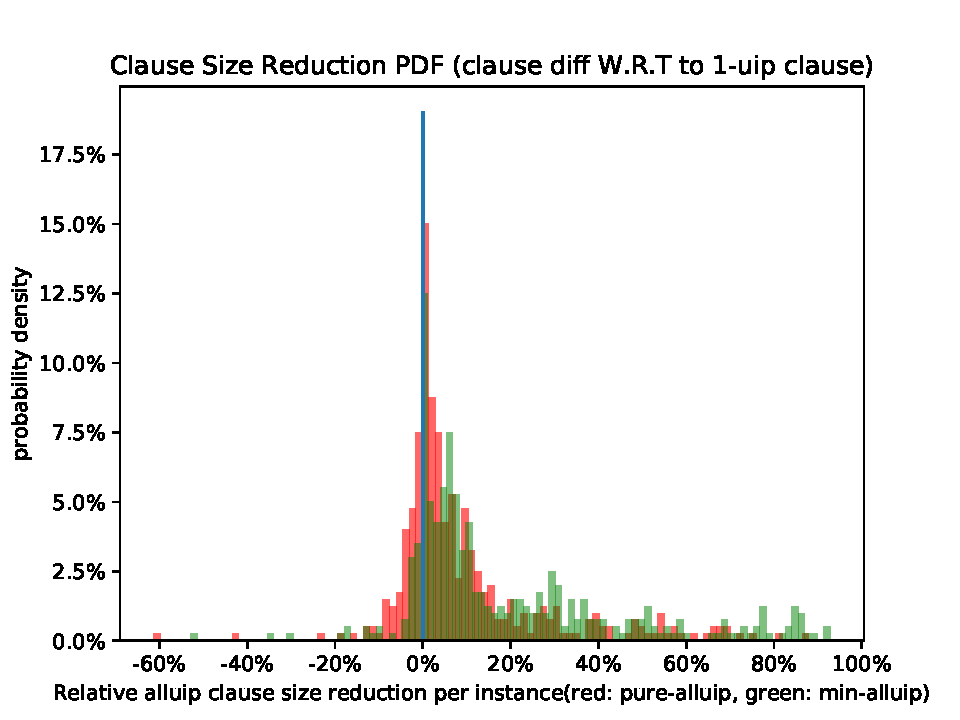
\includegraphics[width=0.8\textwidth]{figures/clause_reduction_PDF}
    \caption{ Relative clause size reduction distribution. X axis
      indicates the relative size of difference between i-uip and
      1-uip clauses (calculated as
      $\dfrac{|\oneUIPClause|-|\iUIPClause|}{|\oneUIPClause|}$ ) for
      each instance, and Y axis shows the probability density.}
     \label{fig:len_pdf}
\end{figure}
\begin{figure} \label{fig:len_compare}
    \centering
    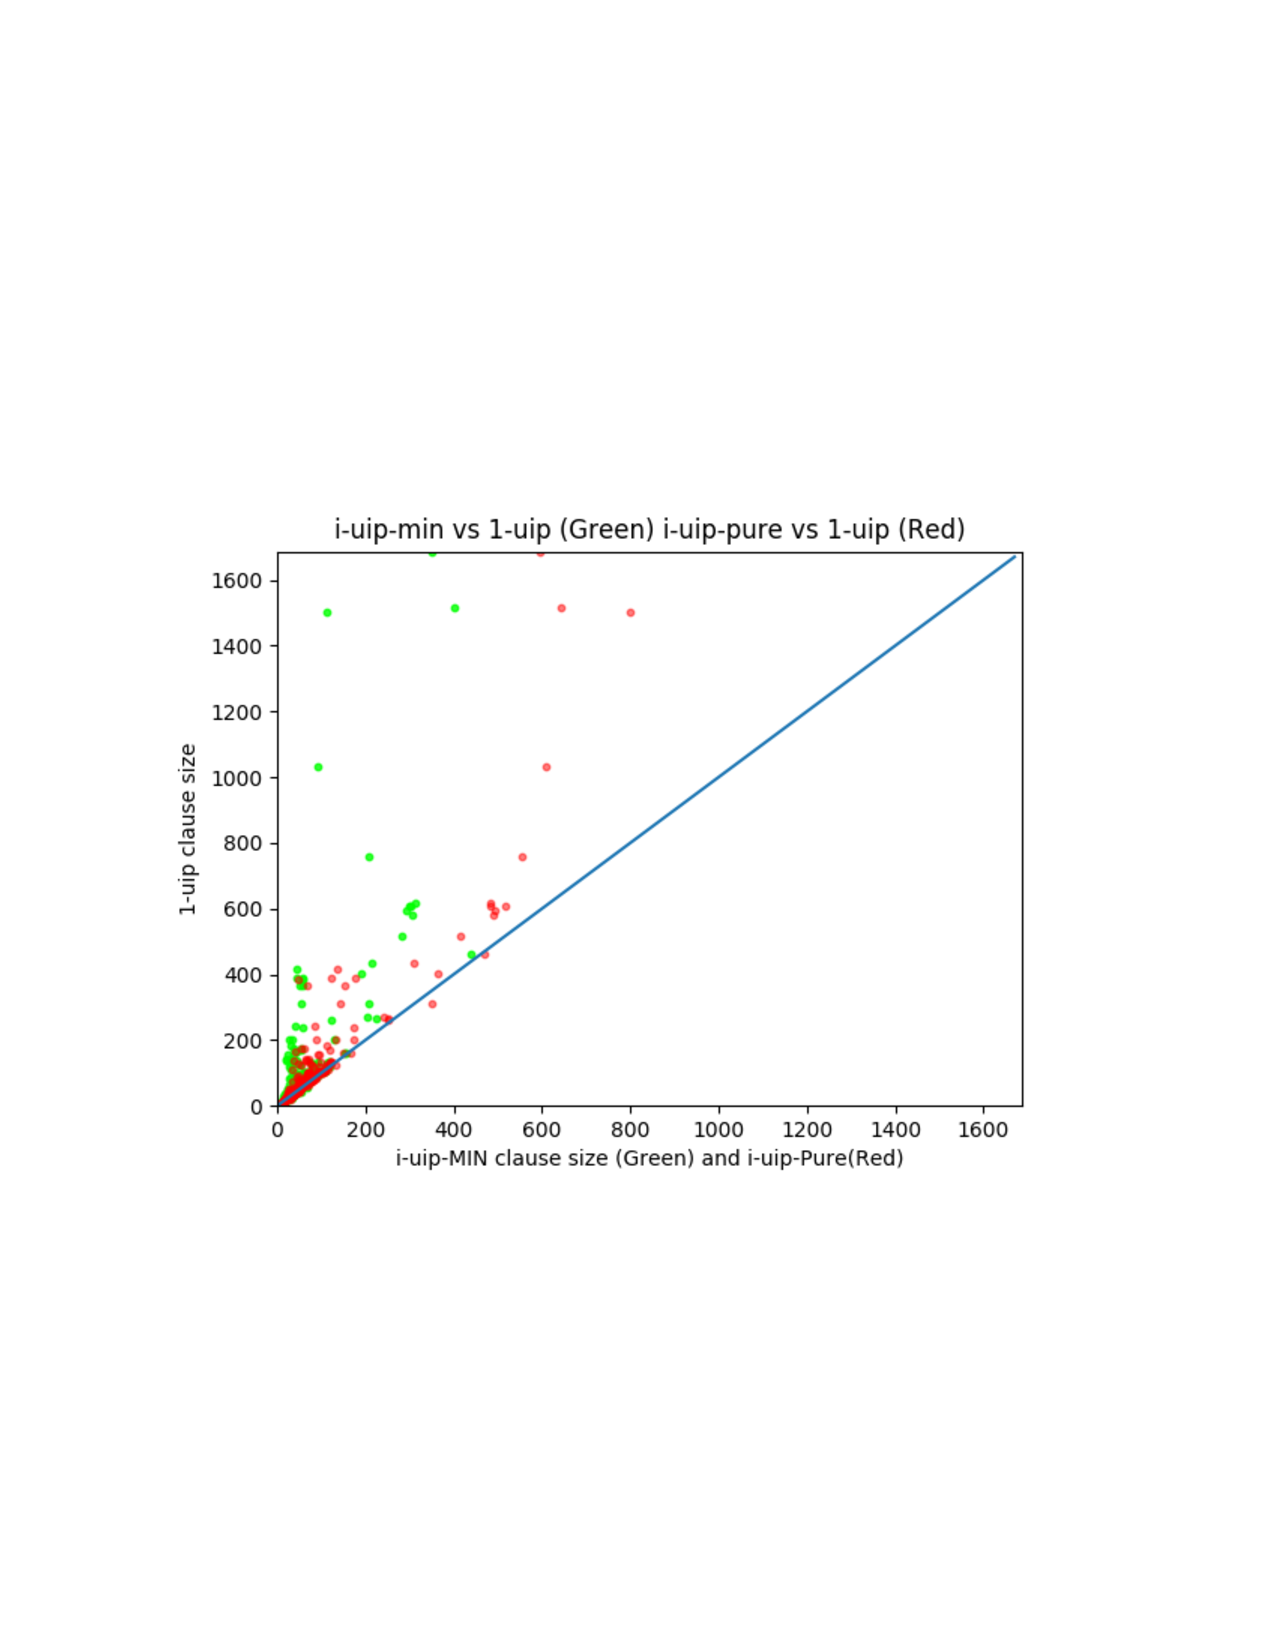
\includegraphics[width=0.8\textwidth]{figures/i-uip-sizes-compare.pdf}
    \caption{Average clause size comparison plot. Each point in the
      plot represents an instance. X and Y axis shows the clause
      length from $\IUIP$ and 1-UIP, respectively. Each green (red)
      dot represents an compared instance between $\MapleBase$ and
      $\MapleIUIMIN$ ($\IUIPPURE$). }
    \label{fig:len_compare}
\end{figure}
\nf{ Do we need this?  We additionally looked at the 14 instances
  solved by $\IUIPMIN$ but not by 1-UIP. $\IUIPMIN$ produces smaller
  clauses for all of them with average relative reduction of 22\% and
  maximum 77\% (30 vs 135). Seven out of 14 instances has size
  relative reduction over 30\%. For the 9 instances solved by 1-UIP
  but not by $\IUIPMIN$, $\IUIPMIN$ only produce smaller clause for
  three instances and with average relative reduction of 3.3\%.}

$\IUIPMIN$ outperformed $\IUIPPURE$ in clause size.  This results agrees with our observation in Fig.~\ref{fig:t2}: $\IUIPMIN$ attempted $\IUIP$ learning more frequently, and it is more likely to succeed.  

\begin{figure} 
\begin{center} 
\begin{tabular}{ | m{3.5cm} | m{5cm}| m{3.5cm} | } 
\hline
Solver & $\IUIP$ attempt rate & $\IUIP$ success rate  \\ 
\hline
$\MapleIUIPPURE$ & 16.1\% & 43.4\% \\ 
\hline
$\MapleIUIMIN$ & 28.8\% & 59.3\% \\ 
\hline
\end{tabular}
\end{center}
\caption{Compare $\IUIPPURE$ and $\IUIPMIN$ i-uip attempt rate and success rate. $\IUIPMIN$ scheme attempted $\IUIP$ more frequently, and it is more likely to successfully produce smaller $\iUIPClause$ clause .}
\label{fig:t2}
\end{figure}

A solver produce smaller clauses can construct smaller proofs. For
UNSAT instances, we measure their DRUP\cite{} proof checking time as
well as the size of the optimized DRUP proof. We used DART-trim
\cite{} with 5000 timeout to check and optimize DRUP proofs.

Fig.~\ref{fig:t3} shows that the optimized proof construct by
$\IUIPMIN$ and $\IUIPPURE$ are significantly smaller than 1-UIP
proofs. The relative proof size reduction roughly correlates to the
average clause size reduction. Fig.~\ref{fig:proof_compare} shows the
absolute proof size comparison results.

\begin{figure} 
\begin{center} 
\begin{tabular}{ | m{3.5cm} | m{5cm}| m{3.5cm} | } 
\hline
Solver & optimized proof size (MB) & relative reduction size  \\ 
\hline
$\MapleBase$ & 613.9 & 0  \\ 
\hline
$\MapleIUIPPURE$ & 487.2 & 6.90\% \\ 
\hline
$\MapleIUIMIN$ & 413.2 & 17.18\% \\ 
\hline
\end{tabular}
\end{center}
\caption{Optimized UNSAT proof comparison for 1-UIP $\IUIPPURE$ and $\IUIPMIN$. Optimized proof size measures the average absolute proof size in MB, and relative reduction size measures the average relative reduction for all UNSAT instances.}
\label{fig:t3}
\end{figure}

\begin{figure}
    \centering
    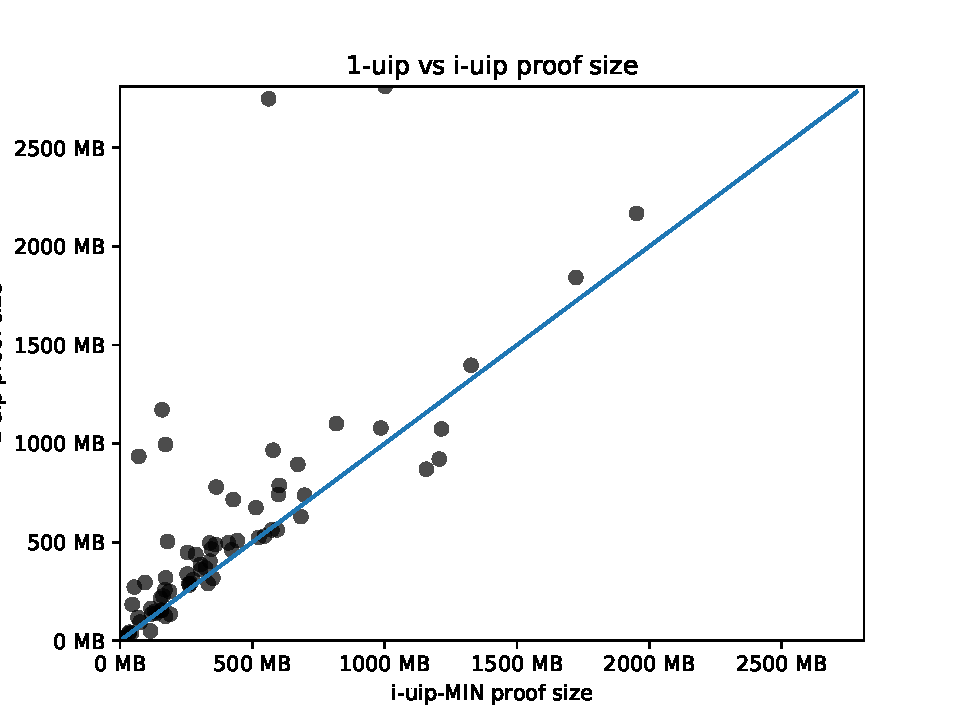
\includegraphics[width=0.8\textwidth]{figures/proof_size_compare.pdf}
    \caption{Average optimized proof size between 1-uip and $\IUIPMIN$.}
    \label{fig:proof_compare}
\end{figure}


\begin{figure} 
\begin{center}
\begin{tabular}{ | m{3.5cm} | m{4cm}| m{2cm} | m{2.75cm} |  } 
\hline
Solver & \# solved (SAT, UNSAT) & PAR-2 & Avg clause Size \\ 
\hline
1-UIP & 221 (132, 89)  & 5018.89 & 62.6  \\ 
\hline
\nf{$\IUIPPURE$} &\textbf{228} (135, \nf{93}) & 4867.37 & 49.88 \\
\hline
$\IUIPMIN$ & 226 (135, 91) & 4890.67 & 45.2 \\ 
\hline
$\IUIPGreedy$ & 226 (135, 91)  & \textbf{4866.94} & 47.7 \\
\hline
$\IUIPActive$ & 225 (\textbf{138}, 87) & 4958.49 & 52..12 \\
\hline
$\IUIPDist$ & 223 (134, 89) & 5015.23 & \textbf{43.2} \\
\hline
\end{tabular}
\end{center}
\caption{Benchmark results of $\MapleBase$ with 1-UIP, $\IUIPPURE$, $\IUIPMIN$, $\IUIPGreedy$,
$\IUIPActive$, and $\IUIPDist$ on SAT2019 race main track.}
\label{fig:t4}
\end{figure}

\subsection{$\IUIP$ as a Practical Learning Scheme}
To evaluate $\IUIP$'s effectiveness as a clause learning scheme, we
re-implement $\IUIPMIN$ on $\MapleBase$ with the extensions mentioned
in section~\ref{sec:i-uip}. We evaluated 1-UIP learning and five
$\IUIP$ configurations ( $\IUIPMIN$, $\IUIPPURE$, $\IUIPGreedy$,
$\IUIPActive$, and $\IUIPDist$) on the SAT Race 2019 main track
benchmark and reported solved instances, PAR-2 score and average
clause size.

Fig.~\ref{fig:t4} summarizes the result of the experiment. Learning
scheme $\IUIPPURE$ solved the most overall instances (228) and the
most UNSAT instances (93). $\IUIPGreedy$ had the lowest PAR-2
score. $\IUIPActive$ solved the most SAT instances (138). $\IUIPDist$
produced the shortest average clause size, but solved the second least
instances, one more instance than the baseline 1-UIP learning. All
configurations of $\IUIP$ outperformed the baseline 1-UIP scheme in
solved instances, PAR-2 score and average clause size.


\subsection{$\IUIP$ on Modern SAT solvers}
To validate $\IUIP$ as a generalizable learning scheme on modern SAT
solvers, we re-implement $\IUIP$ on the winners of 2017, 2018 and 2019
SAT Race\cite{} and $\expSAT$\cite{} ($\expSATShort$). $\expSATShort$
is a top ten solver from 2019 SAT race which uses random walk
simulation to help branching. We chose $\expSATShort$ because 1) it is
a top solver in the 2019 SAT Race without using chronological
backtracking; 2) the combination of random walk simulation and
variable activity branching heuristic allows our learning schemes to
partially sidestep the problem of variable activity. For each solver,
we compare the base 1-UIP learning scheme against $\IUIPPURE$,
$\IUIPMIN$ and the top two $\IUIP$ variants, $\IUIPGreedy$ and
$\IUIPActive$, on the SAT Race 2019 main track benchmark. We report
solved instances, PAR-2 score and the average clause size.

\begin{figure} 
\begin{center}
\begin{tabular}{ | m{3.7cm} | m{4cm}| m{2cm} | m{2.75cm} |  } 
\hline
Solver & \# solved (SAT, UNSAT) & PAR-2 & Avg clause Size \\ 
\hline
SAT 2017 Winner & & & \\
$\MapleSeven$ & 232 (135, 97) & 4755.96 & 61.9  \\ 
\hline
$\MapleSeven$-i-pure & \textbf{244 (146, 98)} +12 & \textbf{4504.18} & 43.76 \\
\hline
$\MapleSeven$-i-min & 240 (144, 96) +8 & 4601.25 & \textbf{36.97} \\ 
\hline
$\MapleSeven$-i-greedy & 237 (140, 97) +5 & 4678.434 & 43.62 \\ 
\hline
$\MapleSeven$-i-inclusive & 234 (137, 97) +2 & 4718.03 & 37.96 \\
\hline
\hline
SAT 2018 Winner & & & \\
$\MapleEightShort$ & 236 (138, 98) & 4671.81 & 61.69 \\
\hline
$\MapleEightShort$-i-pure & \textbf{241} (\textbf{142, 99}) +5 & \textbf{4598.18} & 44.19 \\
\hline
$\MapleEightShort$-i-min & 236 (141, 95) +0 & 4683.92 & 38.05 \\ 
\hline
$\MapleEightShort$-i-greedy & 240 (141, \textbf{99}) +4 & 4626.99 & 41.16 \\
\hline
$\MapleEightShort$-i-inclusive & 240 (\textbf{142}, 98) +4 & 4602.13 & \textbf{37.52} \\
\hline
\hline
SAT 2019 Winner & & & \\
$\MapleNineShort$ & 238 (140, \textbf{98}) & 4531.24 & 60.91 \\
\hline
$\MapleNineShort$-i-pure & 238 (140, \textbf{98}) +0 & 4519.08 &  43.32\\
\hline
$\MapleNineShort$-i-min & 244 (\textbf{148}, 96) +6 & \textbf{4419.84} & \textbf{36.88} \\
\hline
$\MapleNineShort$-i-greedy & 243 (146, 97) + 5 & 4476.73 & 40.65 \\
\hline
$\MapleNineShort$-i-inclusive & \textbf{243} (\textbf{148}, 95) +5 & 4455.76 & 37.02 \\
\hline
\hline
SAT 2019 Competitor & & &\\
$\expSATShort$ & 237 (137, 100)  & 4628.96 & 63.19 \\
\hline
$\expSATShort$-i-pure & 235 (136, 99) -2  & 4668.96 & 48.26 \\
\hline
$\expSATShort$-i-min & 241 (143, 98) +4 & 4524.28 & 46.29 \\ 
\hline
$\expSATShort$-i-greedy & 244 (143, \textbf{101}) +7 & \textbf{4460.92} & 47.25 \\
\hline
$\expSATShort$-i-inclusive & \textbf{245} (\textbf{146}, 99) +8 & 4475.76 & \textbf{45.33} \\
\hline
\end{tabular}
\end{center}
\caption{Benchmark results of 1-UIP, $\IUIPPURE$. $\IUIPMIN$, $\IUIPGreedy$ and $\IUIPActive$ on SAT2019 race main track.}
\label{fig:t5}
\end{figure}

Table~\ref{fig:t5} shows the benchmark result of $\IUIP$
configurations on different solvers. All four configurations of
$\IUIP$ outperformed 1-UIP learning for the SAT 2017 race winner,
$\MapleSeven$. More specifically, $\IUIPPURE$, $\IUIPMIN$,
$\IUIPGreedy$ and $\IUIPActive$ solved 12, 8, 5 and 2 more instances,
respectively, whiling producing smaller clauses. $\IUIPPURE$ solved
more UNSAT and SAT instances while other configurations improved on
solving SAT instances.  The improvement of $\IUIP$ is more significant
on $\MapleSeven$ than on $\MapleBase$ for both solved instances and
clause size reduction. This may suggests that $\IUIP$ and the recent
learnt clause minimization approach~\cite{} synergies well because
i-UIP clauses are shorter with more common literals which allows
vivification~\cite{} to prune literals more aggressively through unit
propagation.

We observed significant improvement of $\IUIP$ for the SAT 2018
winner, $\MapleEightShort$. Three out of four $\IUIP$ configurations
outperformed 1-UIP by 5, 4 an 4 instances,
respectively. $\MapleEightShort$ improved from $\MapleSeven$ by using
chronological backtracking (CB) for long distance
backtracks. Therefore, we used $\IUIP$-CB extension for all $\IUIP$
configurations. The results indicates that the improvement of $\IUIP$
is slightly shadowed by the adoption of CB. More specifically, we
believe CB prevents decision levels from being compressed through the
process of backtracking and literal assertion. The shorter i-UIP
clauses can bring related literals closer, which in turns compresses
the assertion stack and the decision levels. However, since CB
discourages long distance backtracking, the effect of learning shorter
clauses is shadowed until a full restart.  We believe we have observed
an interesting interaction effect that shows the limitations of both
CB and $\IUIP$ learning for future research.

$\IUIP$ learning schemes showed significant improvement for
$\MapleNineShort$. Three out of four configurations improved solved
instances by 6, 5 and 5 instances, respectively. $\MapleNineShort$
uses duplicate learning (DL) to prioritize clauses that are learned
multiple times. $\IUIP$ and DL didn't synergies well possibly because
i-UIP clauses are less likely to be duplicated. We observed that
$\IUIPMIN$ ,in average, added 12\% less duplicated clauses into the
core clause database than 1-UIP. One possible explanation is that
$\IUIP$ learning can reduce an 1-UIP clause to different i-UIP clauses
for different assertion trails. Therefore, the solver is less likely
to learn the same i-UIP clauses.

We observed significant improvement of $\IUIP$ for $\expSATShort$,
three out of four configurations of $\IUIP$ significantly outperformed
1-UIP learning by 4, 7 and 8 more instances, respectively, while
producing smaller clauses. We expect all three configurations of
$\IUIP$ to solve the similar amount of instances with close PAR-2
scores because the additional random walk exploration allows the
learning schemes to partially sidestep the activity problem; hence,
the learning adjustment for variable activities should have less
impact on the solver's performance. However, we instead, observed that
both $\IUIPGreedy$ and $\IUIPActive$ outperformed the default i-UIP
learning scheme. One possible explanation is that $\IUIPGreedy$ and
$\IUIPActive$ schemes could easily overcompensate variable activities
for i-UIP clauses, and $\expSATShort$'s random walk exploration could
use future search information to mitigate the negative effects of our
overcompensation.

\bibliography{sat}{}
\bibliographystyle{splncs04}
\end{document}

